% !TeX root = surprises.tex

\chapter{Construcción de un Heptadecágono regular}\label{c.heptadecagon}

%%%%%%%%%%%%%%%%%%%%%%%%%%%%%%%%%%%%%%%%%%%%%%%%%%%%%%%%%%%%%%%

Los únicos polígonos regulares que los griegos sabían construir con regla y compás eran el triángulo, el cuadrado, el pentágono y el polígono regular de $15$ lados. Dado un polígono regular de $n$ lados, se puede construir un polígono de $2n$ lados circunscribiendo el polígono en una circunferencia y bisecando el ángulo central (Fig.~\ref{f.hept-double}). No se hicieron más progresos hasta 1796, cuando Carl Friedrich Gauss se despertó una mañana, justo antes de cumplir 19 años, y mediante <<pensamiento concentrado>> descubrió cómo construir un \emph{heptadecágono} regular, un polígono regular con $17$ lados. Este logro le inspiró para convertirse en matemático.

En la sección~\ref{s.hept-regular} se analiza la relación entre el lado de un polígono inscrito en una circunferencia y el ángulo central que subtiende. En la sección~\ref{s.fundamental} se expone sin demostraciones el Teorema Fundamental del Álgebra. Sección~\ref{s.roots} presenta las raíces de la unidad, las raíces del polinomio $x^n-1$, que son fundamentales para la demostración de Gauss. Las secciones~\ref{s.gauss} y~\ref{s.derivation} presentan la demostración de Gauss que se basa en simetrías de raíces de polinomios. Gauss derivó una fórmula que demuestra que el heptadecágono es construible, pero no se dio una construcción geométrica hasta casi un siglo después. La sección~\ref{s.construction} ofrece una elegante construcción de James J. Callagy. La sección~\ref{s.hept-pentagon} muestra cómo las construcciones de un pentágono regular se pueden derivar utilizando tanto la geometría como la trigonometría.

Parte del material es más sencillo si se presenta utilizando números complejos. Este material se establece en /los recuadros que se pueden omitir.
\begin{figure}[b]
\begin{center}
\begin{tikzpicture}[scale=.4]
\coordinate (O) at (0,0);
\vertex{O};
\foreach \x/\name/\n/\po in {0/a/A/right,1/b/B/above,2/c/C/left,3/d/D/below left,4/e/E/below right} {
  \coordinate (\name) at ($(O)+(\x*72+18:3cm)$);
}
\draw (a) -- (b) -- (c) -- (d) -- (e) -- (a);
\node[draw,circle through=(a)] at (O) {};
\draw (d) -- (O) -- (e);
\draw [very thick,dotted] (O) -- (-90:3) -- (e) -- (-90:3) -- (d);
\end{tikzpicture}
\end{center}
\caption{Construcción de un polinomio regular de $10$ lados a partir de un pentágono regular}\label{f.hept-double}
\end{figure}

\section{Construcción de polígonos regulares}\label{s.hept-regular}

La construcción del heptadecágono regular condujo al teorema de Gauss-Wantzel, que afirma que un polígono regular con $n$ lados se puede construir con una regla y un compás si y sólo si $n$ es el producto de una potencia de $2$ y cero o más números de Fermat $2^{2^k}+1$ que son primos. Los números primos de Fermat conocidos son:
\[
F_0=3,\quad F_1=5,\quad F_2=17,\quad F_3=257,\quad F_4=65,537\,.
\]
Un polígono regular con $257$ lados fue construido por Magnus Georg Paucker en $1822$ y por Friedrich Julius Richelot en $1832$. En $1894$ Johann Gustav Hermes afirmó haber construido un polígono regular con $65,537$ lados.

Para construir un polígono regular basta con construir un segmento de longitud $\cos \theta$, donde $\theta$ es el ángulo central subtendido por una cuerda que es un lado del polígono inscrito en un círculo unitario. Dado el segmento $\overline{OB}=\cos\theta$, construimos una perpendicular en $B$ y denotamos con $C$ su intersección con la circunferencia unitaria. Entonces:
\begin{eqnarray*}
\cos \theta&=&\displaystyle\frac{\overline{OB}}{\overline{OC}}=\overline{OB}\\
\theta &=& \cos^{-1} (\overline{OB})\,.
\end{eqnarray*}
La cuerda $\overline{AC}$ es un lado del polígono regular (Fig.~\ref{f.hept-central1}).
\begin{figure}[b]
\begin{center}
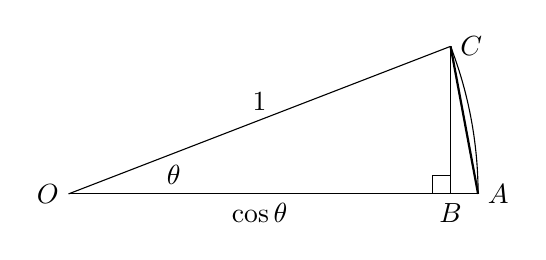
\begin{tikzpicture}[scale=1.3]
\coordinate (O) at (0,0) node[left] {$O$} node[above right,xshift=32pt] {$\theta$};
\coordinate (A) at (4,0);
\node[right] at (A) {$A$};
\draw (O) -- (A);
\draw (A) arc(0:21.12:4);
\coordinate (C) at (21.12:4cm);
\draw (O) -- node[above] {$1$} (C);
\node[right] at (C) {$C$};
\draw (C) -- (C |- A) coordinate (B);
\node[below] at (B) {$B$};
\draw[rotate=90] (B) rectangle +(5pt,5pt);
\draw[thick] (A) -- (C);
\path (O) -- node[below] {$\cos \theta$} (B); 
\end{tikzpicture}
\end{center}
\caption{El coseno del ángulo central de un polígono regular}\label{f.hept-central1}
\end{figure}

Dado un segmento definido como de longitud $1$, las longitudes que son construibles son las que se pueden obtener a partir de segmentos de longitud conocida mediante las operaciones $\{+,-,\times,/,\surd\}$ (Sec.~\ref{s.trisect-constructible}). Gauss demostró que $\cos(360^\circ/17)$, el coseno del ángulo central de un heptadecágono, es construible ya que se puede expresar utilizando sólo estas operaciones:\index{Heptadecagon!cosine of the central angle}
\begin{eqnarray*}
\cos\left(\frac{360^\circ}{17}\right) &=& 
-\frac{1}{16}+\frac{1}{16}\sqrt{17} + 
     \frac{1}{16}\sqrt{34-2\sqrt{17}}
    + \\
    &&
     \frac{1}{8}\sqrt{
     17+3\sqrt{17} - 
     \sqrt{34-2\sqrt{17}}
   -2
     \sqrt{34+2\sqrt{17}}
   }\,.
\end{eqnarray*}

\section{Teorema fundamental del álgebra}\label{s.fundamental}

El siguiente teorema se utilizará sin demostración.

\begin{theorem}\label{thm.fundamental} Todo polinomio de grado $n$ tiene exactamente $n$ raíces.
\end{theorem}\index{Fundamental theorem of algebra}

El enunciado del teorema se ha simplificado porque todo lo que necesitaremos saber es que $n$ raíces \emph{existen}.

\begin{advanced}
\textbf{El Teorema Fundamental del Álgebra} afirma que todo polinomio no constante de grado $n$ en una sola variable con coeficientes \emph{complejos}  tiene exactamente $n$ raíces \emph{complejos}.
Si hay varias raíces con el mismo valor, se cuentan todas: $x^2-4x+4=(x-2)(x-2)$ tiene dos raíces ambas iguales a $2$.
El polinomio $x^2+1$ con coeficientes enteros tiene dos raíces complejas $\pm\sqrt{-1}$.
Curiosamente, aunque el teorema se refiere a entidades algebraicas finitas -polinomios de grado $n$ con $n$ raíces- se necesitan métodos de análisis, normalmente análisis complejo, para demostrar el teorema.
\end{advanced}

\section{Raíces de la unidad}\label{s.roots}

Por el Teorema Fundamental del Álgebra (Teorema~\ref{thm.fundamental}) el polinomio $x^{n}-1$ tiene $n$ raíces para cualquier entero $n> 1$. Una raíz es $x=1$ por lo que hay otras $n-1$ raíces. Denotemos una de estas raíces con $r$. Como $r^{n}=1$ se llama una \emph{enésima raíz de la unidad}. ¿Y $r^2$?
\[
(r^{2})^n=(r^{n})^2=1^2=1\,.
\]
Se deduce que los números $n$:
\[
1, r, r^2, \ldots, r^{n-2}, r^{n-1}
\]
son $n$-ésimas raíces de la unidad.

\begin{advanced}
Sea $r=\cos \left(\frac{2\pi}{n}\right) + i\sen  \left(\frac{2\pi}{n}\right)$.
Por la fórmula de Moivre:\index{fórmula de Moivre}
\[
\left[\cos \left(\frac{2\pi}{n}\right) + i\sen  \left(\frac{2\pi}{n}\right)\right]^{n}=
\cos \left(\frac{2 n\pi}{n}\right) + i\sen  \left(\frac{2 n\pi}{n}\right)= 1\,.
\]
\vspace*{-3ex}
\end{advanced}

\begin{theorem}
Sea $n$ un \emph{número primo} y sea $r$ una raíz enésima de la unidad. Entonces:
\[
\{1,r,r^2,\ldots,r^{n-2},r^{n-1}\}
\]
son distintos por lo que son \emph{todas} las enésimas raíces de la unidad.
\end{theorem}

\begin{proof}
Supongamos que las potencias no son distintas de modo que $r^i=r^j$ para algún $0\leq i<j\leq n-1$. Entonces $r^j/r^i=r^{j-i}=1$ por lo que existe al menos un entero positivo $i'$ menor que $n$ tal que $r^{i'}=1$. Sea $m$ el menor de dichos enteros positivos. Por el algoritmo de la división de enteros $n=ml+k$ para algún $0<l<n$ y $0\leq k<m$. De:
\[
1=r^n=r^{ml+k}=(r^m)^l\cdot r^k=1^l\cdot r^k=r^k\,,
\]
tenemos $0\leq k<m$ y $r^k=1$. Dado que $m$ se definió como el menor entero positivo $k=0$ y $n=ml$ no es primo.
\end{proof}

\begin{theorem} Sean $\{a_1,a_2,\ldots,a_{n-1},a_n\}$ las raíces de un polinomio de enésimo grado $f(x)$. Entonces:
\begin{align}\label{eq.viete}
f(x) =(x-a_1) (x-a_2)\cdots (x-a_{n-1})(x-a_n)\,.
\end{align}
\end{theorem}

\begin{proof}
Si $a_i$ es una raíz de $f(x)$ por definición $f(a_i)=0$ pero:
\begin{eqnarray*}
f(a_i)&=&(a_i-a_1) (a_i-a_2)\cdots (a_i-a_{n-1})(a_i-a_n)\\
&=&\cdots (a_i-a_i) \cdots =0\,.
\end{eqnarray*}
Por lo tanto, $f(x)=(x-a_i)g_i(x)$ para algún $g_i(x)$ y por inducción esto vale para todas las raíces.
\end{proof}

A partir de la Ecuación~\ref{eq.viete} es fácil ver que el coeficiente de $x^{n-1}$ es:
\[
-(a_1+a_2+\cdots+a_{n-1}+a_n)\,.
\]
Dado que el coeficiente de $x^{n-1}$ en $x^n-1$ para $n\geq 2$ es cero, tenemos:
\begin{eqnarray*}
-(1+r+r^2+\cdots + r^{n-2}+r^{n-1})&=&0\\
r+r^2+\cdots + r^{n-2}+r^{n-1}&=&-1\,.
\end{eqnarray*}
Para el heptadecágono esto es:
\begin{multline}
r+r^2+r^3+r^4+r^5+r^6+r^7+r^8+\\
r^9+r^{10}+r^{11}+r^{12}+r^{13}+r^{14} + r^{15}+r^{16}=-1.\label{eq.minus-one}
\end{multline}

\section{Prueba de Gauss de que un heptadecágono es construible}\label{s.gauss}

Lo que Gauss entendió es que no es necesario trabajar con las raíces en su orden natural $r,r^2,\ldots,r^{16}$. Los $3^0, 3^1, 3^2, \ldots$ potencias de $r$ dan todas las raíces pero en un orden diferente:
\[
\begin{array}{l}
r^1, \;r^{1\cdot 3 =3},\; r^{3\cdot 3=9},\; r^{9\cdot 3=27=10},\; r^{10\cdot 3=30=13},\; r^{13\cdot 3=39=5},\; r^{5\cdot 3=15},\; r^{15\cdot 3=45=11},\\\\
r^{11\cdot 3 =33=16}, \;r^{16\cdot 3=48=14},\; r^{14\cdot 3=42=8},\; r^{8\cdot 3=24=7},\;r^{7\cdot 3=21=4},\; r^{4\cdot 3=12},\; r^{12\cdot 3=36=2},\; r^{2\cdot 3=6}\,,
\end{array}
\]
donde las raíces han sido reducidas modulo $17$:
\[
r^{17m+k}=(r^{17})^m\cdot r^k=1^m\cdot r^k=r^k\,.
\]
Corroboramos que la lista contiene todas las raíces (excepto $1$) exactamente una vez:
\begin{align}\label{eq.roots}
r^1, r^3, r^9, r^{10}, r^{13}, r^5, r^{15}, r^{11}, r^{16}, r^{14}, r^8, r^7, r^4, r^{12}, r^2, r^6\,.
\end{align}
Dado un polinomio cuadrático monicó cuyas raíces son $a,b$:
\[
y^2+py+q=(y-a)(y-b)=0\,,
\]
podemos calcular los coeficientes $p,q$ a partir de las raíces (Capítulo~\ref{c.quadratic}):
\[
p=-(a+b)\,,\quad q=ab\,.
\]
Por lo tanto, \emph{dado} $a+b$ y $ab$ podemos escribir la ecuación cuadrática de la que $a,b$ son las raíces.

Sea $a_0$ la suma de las raíces en las posiciones impares de la Ecuación~\ref{eq.roots}:
\[
a_0=r + r^9 + r^{13} +r^{15} +r^{16} + r^8+r^4+r^2\,,
\]
y sea $a_1$ la suma de las raíces en las posiciones pares de la Ecuación~\ref{eq.roots}:
\[
a_1=r^3 + r^{10} + r^{5} +r^{11} +r^{14} + r^7+r^{12}+r^6\,.
\]
Para obtener $a_0,a_1$ como raíces de una ecuación cuadrática primero se calcula su suma y se utiliza la Ecuación~\ref{eq.minus-one}:
\[
a_0+a_1=r + r^2 + \cdots +r^{16}=-1\,.
\]
Ahora tenemos que trabajar mucho para calcular su producto. La figura muestra el cálculo donde los valores de $r^ir^j=r^{i+j}$ se escriben después de reducir los exponentes modulo $17$. Comprobamos que cada raíz se produce exactamente cuatro veces para que - de nuevo utilizando Ecuación~\ref{eq.minus-one} - el valor del producto es $-4$.

\begin{figure}[t]
\[
\renewcommand{\arraystretch}{1.6}
\begin{array}{lcl}
a_0a_1&=&(r + r^9 + r^{13} +r^{15} +r^{16} + r^8+r^4+r^2)\;\;\times\\
&&(r^3 + r^{10} + r^{5} +r^{11} +r^{14} + r^7+r^{12}+r^6)\\
&=&\occ{4}{1} + \occ{11}{1} + \occ{6}{1} + \occ{12}{1} + \occ{15}{1} + \occ{8}{1} + \occ{13}{1} + \occ{7}{1} +\\
&&\occ{12}{2} + \occ{2}{1} + \occ{14}{1} + \occ{3}{1} + \occ{6}{2} + \occ{16}{1} + \occ{4}{2} + \occ{15}{2} +\\
&&\occ{16}{2} + \occ{6}{3} + \occ{1}{1} + \occ{7}{2} + \occ{10}{1} + \occ{3}{2} + \occ{8}{2} + \occ{2}{2}\;\;\: +\\
&&\occ{1}{2} + \occ{8}{3} + \occ{3}{3} + \occ{9}{1} + \occ{12}{3} + \occ{5}{1} + \occ{10}{2} + \occ{4}{3}\;\;\: +\\
&&\occ{2}{3} + \occ{9}{2} + \occ{4}{4} + \occ{10}{3} + \occ{13}{2} + \occ{6}{4} + \occ{11}{2} + \occ{5}{2} \:+\\
&&\occ{11}{3} + \occ{1}{3} + \occ{13}{3} + \occ{2}{4} + \occ{5}{3} + \occ{15}{3} + \occ{3}{4} + \occ{14}{2} \;+\\
&&\occ{7}{3} + \occ{14}{3} + \occ{9}{3} + \occ{15}{4} + \occ{1}{4} + \occ{11}{4} + \occ{16}{3} + \occ{10}{4} +\\
&&\occ{5}{4} + \occ{12}{4} + \occ{7}{4} + \occ{13}{4} + \occ{16}{4} + \occ{9}{4} + \occ{14}{4} + \occ{8}{4}\\
&=&-4\,.
\end{array}
\]
\caption{Cálculo de $a_0a_1$; debajo de cada raíz está el número de apariciones de la raíz hasta el momento}\label{fig.a0a1}
\end{figure}

Como $a_0+a_1=-1$ y $a_0 a_1=-4$, $a_1,a_2$ son las raíces de la ecuación cuadrática $y^2+y-4=0$ y se pueden calcular mediante la fórmula simple de las raíces de una ecuación cuadrática:
\[
a_{0,1} = \frac{-1\pm\sqrt{17}}{2}\,.
\]
Ahora bien, sean $b_0,b_1,b_2,b_3$ las sumas de cada cuarta raíz a partir de $r^1,r^3,r^9,r^{10}$, respectivamente:
\begin{eqnarray*}
b_0&=& r^1+ r^{13} + r^{16} + r^4\\
b_1&=& r^3+ r^{5} + r^{14} + r^{12}\\
b_2&=& r^9+ r^{15} + r^{8} + r^2\\
b_3&=& r^{10}+ r^{11} + r^{7} + r^6\,.
\end{eqnarray*}%
Corroboramos que $b_0+b_2=a_0, b_1+b_3=a_1$ y calcula los productos correspondientes (Fig.~\ref{f.b0213}).
\begin{figure}[t]
\begin{eqnarray*}
b_0b_2&=&(r + r^{13} + r^{16} +r^4)\;\;\times\;(r^9 + r^{15} + r^{8} +r^{2})\\
&=&(r^{10}+r^{16}+r^9+r^3)\,+\;\,(r^{5}+r^{11}+r^4+r^{15})+\\
&&(r^{8}+r^{14}+r^7+r^1)\,\;\,+\;\,(r^{13}+r^{2}+r^{12}+r^6)\\
&=&-1\\
%\end{eqnarray*}%
%\begin{eqnarray*}
b_1b_3&=&(r^3 + r^{5} + r^{14} +r^{12})\;\;\times\;(r^{10} + r^{11} + r^{7} +r^{6})\\
&=&(r^{13}+r^{14}+r^{10}+r^9)\;+\;(r^{15}+r^{16}+r^{12}+r^{11})+\\
&&(r^{7}+r^{8}+r^4+r^3)\quad\;\, +\;(r^{5}+r^{6}+r^{2}+r^1)\\
&=&-1\,.
\end{eqnarray*}%
\caption{Cálculo de $b_0b_2,b_1b_3$}\label{f.b0213}
\end{figure}
Para resumir estos cálculos:
\begin{eqnarray*}
b_0+b_2&=&a_0\\
b_0b_2&=&-1\\
b_1+b_3&=&a_1\\
b_1b_3&=&-1\,,
\end{eqnarray*}%
por lo que $b_0,b_2$ son las soluciones de $y^2-a_0y-1= 0$, y $b_1,b_3$ son las soluciones de $y^2-a_1y-1 =0$. Utilizando los valores calculados anteriormente para $a_0,a_1$ podemos calcular las raíces $b_0,b_1$ (Fig.~\ref{f.b0b1}).
\begin{figure}[t]
\begin{eqnarray*}
b_0&=&\frac{a_0+\sqrt{a_0^2+4}}{2}\\
&=&\frac{
     \displaystyle\frac{(-1+\sqrt{17})}{2} + 
     \sqrt{\left(\displaystyle\frac{(-1+\sqrt{17})}{2}\right)^2+4}
   }{2}\\
&=&\frac{
     (-1+\sqrt{17}) + 
     \sqrt{\left(-1+\sqrt{17}\right)^2+16}
   }{4}\\
&=&\frac{
     (-1+\sqrt{17}) + 
     \sqrt{34-2\sqrt{17}}
   }{4}\\
b_1&=&\frac{a_1+\sqrt{a_1^2+4}}{2}\\
&=&\frac{
     \displaystyle\frac{(-1-\sqrt{17})}{2} + 
     \sqrt{\left(\displaystyle\frac{(-1-\sqrt{17})}{2}\right)^2+4}
   }{2}\\
&=&\frac{
     (-1-\sqrt{17}) + 
     \sqrt{\left(-1-\sqrt{17}\right)^2+16}
   }{4}\\
&=&\frac{
     (-1-\sqrt{17}) + 
     \sqrt{34+2\sqrt{17}}
   }{4}\,.
\end{eqnarray*}
\caption{Cálculo de $b_0$ y $b_1$}\label{f.b0b1}
\end{figure}

\noindent{}Por último, sean $c_0,c_4$ las sumas de cada raíz octava a partir de $r^1,r^{13}$:
\begin{eqnarray*}
c_0&=&r^1+r^{16}\\
c_4&=&r^{13}+r^4\\
c_0+c_4&=&r^1+r^{16}+r^{13}+r^4=b_0\\
c_0c_4&=&(r^1+r^{16})\cdot(r^{13}+r^4)\\
&=&r^{14}+r^5+r^{12}+r^3=b_1\,,
\end{eqnarray*}
por lo que $c_0,c_4$ son las raíces de $y^2-b_0y+b_1=0$. Como $\cos(360^\circ/17) = c_0/2$ (Fig.~\ref{f.hept-cosine}) basta calcular la raíz $c_0=r^1+r^{16}$ (Fig.~\ref{fig.c0}).

\begin{figure}[b]
\begin{center}
\begin{tikzpicture}[scale=1]
\coordinate (O) at (0,0) node[left] {$O$}
  node[above right,xshift=20pt] {$\theta$}
  node[below right,xshift=20pt] {$\theta$};
\coordinate (A) at (4,0);
\coordinate (C) at (21.12:4cm);
\coordinate (D) at (-21.12:4cm);
\draw (D) arc(-21.12:21.12:4);
\draw (D) -- node[below] {$1$} (O) -- node[above] {$1$} (C);
\node[right] at (C) {$r^1$};
\node[right] at (D) {$r^{16}$};
\draw (C) -- (C |- A) coordinate (B);
\draw (D) -- (D |- A);
\draw[rotate=90] (B) rectangle +(5pt,5pt);
\draw (D) -- (A) -- (C);
\draw[<->] ($(O)+(3pt,0)$) --
  node[fill=white] {$\cos \theta$} (B);
\end{tikzpicture}
\end{center}
\caption{El coseno del ángulo central calculado a partir de $r_1,r_{16}$}\label{f.hept-cosine}
\end{figure}

\begin{figure}[t]
\begin{eqnarray*}
c_0&=&\frac{b_0+\sqrt{b_0^2-4b_1}}{2}\\
&=&\frac{1}{2}
     \frac{
     (-1+\sqrt{17}) + 
     \sqrt{34-2\sqrt{17}}
   }{4}\,+ \\
&& 
    \frac{1}{2}
       \sqrt{\left(\frac{
     (-1+\sqrt{17}) + 
     \sqrt{34-2\sqrt{17}}
   }{4}\right)^2-4\left(\frac{
     (-1-\sqrt{17}) + 
     \sqrt{34+2\sqrt{17}}
   }{4}\right)}
   \\
&=&-\frac{1}{8}+\frac{1}{8}\sqrt{17} + 
     \frac{1}{8}\sqrt{34-2\sqrt{17}}
    + \\
   &&
     \frac{1}{8}\sqrt{
     \left(
     (-1+\sqrt{17}) + 
     \sqrt{34-2\sqrt{17}}
   \right)^2-16\left(
     (-1-\sqrt{17}) + 
     \sqrt{34+2\sqrt{17}}
   \right)}
\\
&=&-\frac{1}{8}+\frac{1}{8}\sqrt{17} + 
     \frac{1}{8}\sqrt{34-2\sqrt{17}}
   \, + \\
   &&
     \frac{1}{8}\sqrt{
     (-1+\sqrt{17})^2 + 
     2(-1+\sqrt{17})\sqrt{34-2\sqrt{17}}+
     (34-2\sqrt{17})
   -}\\
   &&\overline{
     \left((-16-16\sqrt{17}) + 
     16\sqrt{34+2\sqrt{17}}\right)
   }
\\
&=&-\frac{1}{8}+\frac{1}{8}\sqrt{17} + 
     \frac{1}{8}\sqrt{34-2\sqrt{17}}
    \,+ \\
   &&
     \frac{1}{8}\sqrt{
     68+12\sqrt{17} + 
     2(-1+\sqrt{17})\sqrt{34-2\sqrt{17}}
   -16
     \sqrt{34+2\sqrt{17}}
   }
\end{eqnarray*}
\caption{Cálculo de $c_0$}\label{fig.c0}
\end{figure}

El coseno del ángulo central de un heptadecágono es construible con regla y compás ya que se compone sólo de números racionales y de las operaciones $\{+,-,\times,/,\surd\}$:
\begin{flalign}
\cos\left(\frac{360^\circ}{17}\right) &= 
\frac{c_0}{2}\\
&=-\frac{1}{16}+\frac{1}{16}\sqrt{17} + 
     \frac{1}{16}\sqrt{34-2\sqrt{17}}\; +
    \label{eq.not-gauss1}\\
 & \quad\frac{1}{16}\sqrt{
     68+12\sqrt{17} + 
     2(-1+\sqrt{17})\sqrt{34-2\sqrt{17}}
   -16
     \sqrt{34+2\sqrt{17}}
   }\,.\label{eq.not-gauss2}
\end{flalign}
\begin{advanced}
\vspace{-2ex}
\begin{eqnarray*}
r_1+r_{16}&=&\cos\left(\frac{2\pi}{17}\right)+i\sen\left(\frac{2\pi}{17}\right)+\cos\left(\frac{2\cdot 16\pi}{17}\right)+i\sen\left(\frac{2\cdot 16\pi}{17}\right)\\
&=&\cos\left(\frac{2\pi}{17}\right)+i\sen\left(\frac{2\pi}{17}\right)+\cos\left(\frac{-2\pi}{17}\right)+i\sen\left(\frac{-2\pi}{17}\right)\\
&=&2\cos\left(\frac{2\pi}{17}\right)\,.
\end{eqnarray*}
\vspace{-4ex}
\end{advanced}

\section{Derivación de la fórmula de Gauss}\label{s.derivation}

La fórmula anterior para $\cos(360^\circ /17)$ no es la dada por Gauss. Aquí está una derivación de la fórmula de Gauss:

Simplifiquemos $2(-1+\sqrt{17})\sqrt{34-2\sqrt{17}}$:
\begin{eqnarray*}
2(-1+\sqrt{17})\sqrt{34-2\sqrt{17}} &=&
-2\sqrt{34-2\sqrt{17}} +2\sqrt{17}\sqrt{34-2\sqrt{17}}\\
&&+4\sqrt{34-2\sqrt{17}}-4\sqrt{34-2\sqrt{17}}\\
&=&
2\sqrt{34-2\sqrt{17}} +2\sqrt{17}\sqrt{34-2\sqrt{17}}\\
&&-4\sqrt{34-2\sqrt{17}}\\
&=&2(1+\sqrt{17})\sqrt{34-2\sqrt{17}}-4\sqrt{34-2\sqrt{17}}\,.
\end{eqnarray*}
Recordaremos el término $-4\sqrt{34-2\sqrt{17}}$ por ahora y simplificaremos el primer término elevándolo al cuadrado y luego sacando la raíz cuadrada:
\begin{eqnarray*}
2(1+\sqrt{17})\sqrt{34-2\sqrt{17}}&=&
2\sqrt{\left[(1+\sqrt{17})\sqrt{34-2\sqrt{17}}\right]^2}\\
&=&2\sqrt{(18+2\sqrt{17})(34-2\sqrt{17})}\\
&=&2\sqrt{(18\cdot 34-4\cdot17)+\sqrt{17}(2\cdot 34 - 2\cdot 18)}\\
&=&2\cdot 4\sqrt{34+2\sqrt{17}}\,.
\end{eqnarray*}
Sustituyendo los términos se obtiene la fórmula de Gauss:
\begin{eqnarray*}
\cos\left(\frac{360^\circ}{17}\right) &=&
-\frac{1}{16}+\frac{1}{16}\sqrt{17} + 
     \frac{1}{16}\sqrt{34-2\sqrt{17}} \\
    &&
     +\,\frac{1}{16}\sqrt{
     68+12\sqrt{17} + 
     8\sqrt{34+2\sqrt{17}}-4\sqrt{34-2\sqrt{17}}
   -16
     \sqrt{34+2\sqrt{17}}
   }\\
&=&-\frac{1}{16}+\frac{1}{16}\sqrt{17} + 
     \frac{1}{16}\sqrt{34-2\sqrt{17}}\\
&&+\,\frac{1}{8}\sqrt{
     17+3\sqrt{17} - 
     \sqrt{34-2\sqrt{17}}
   -2
     \sqrt{34+2\sqrt{17}}
   }\,.
\end{eqnarray*}

\section{Construcción de un heptadecágono}\label{s.construction}

\index{Construction!hept@of a regular heptadecagon}
\index{Heptadecagon!construction}
Construimos una circunferencia unitaria centrada en $O$ con diámetros perpendiculares $\overline{QP}$ y $\overline{SR}$ (Fig.~\ref{f.hept-construction1}).
\begin{figure}[b]
\begin{center}
\begin{tikzpicture}[scale=1.2]
\clip (-4.3,-1.8) rectangle (4.3,1.9);

\node at (-.2,1.5) {$\cdots$};
\node at (-.2,1.7) {$R$};
\node at (-.2,-1.5) {$\cdots$};
\node at (-.2,-1.7) {$S$};

\coordinate (O) at (0,0);
\draw (O) circle (4cm);
\coordinate (P) at (4,0);
\coordinate (R) at (0,4);
\coordinate (Q) at (-4,0);
\coordinate (S) at (0,-4);
\coordinate (A) at (0,1);
\coordinate (B) at (.78,0);
\coordinate (C) at (-1.28,0);
\draw (P) -- (Q);
\draw (R) -- (S);
\path (O) -- node[left,xshift=2pt,yshift=-4pt] {$\frac{1}{4}$} (A);
\draw (P) -- ($(P)!1.5!(A)$);
\draw (A) -- node[above] {$\frac{\sqrt{17}}{4}$} (P);
\draw (C) -- (A) -- (B);
\foreach \c/\where in {O/below left, P/right, Q/left, R/above, S/below, A/above left, B/below, C/below} {
  \node[\where] at (\c) {$\c$};
}
\draw (O) rectangle(+5pt,+5pt);
%\vertex{O};
\node[below right,xshift=8pt,yshift=-4pt] at (A) {\sm{\alpha}};
\node[below right,xshift=-2pt,yshift=-6pt] at (A) {\sm{\alpha}};
\node[below left,xshift=1pt,yshift=-2pt] at (A) {\sm{\beta}};
\node[below left,xshift=-4pt,yshift=3pt] at (A) {\sm{\beta}};
\draw[<->] ($(C)+(0,-16pt)$) -- node[below] {$\frac{1+\sqrt{17}}{16}$} ($(O)+(0,-16pt)$);
\draw[<->] ($(O)+(0,-16pt)$) -- node[below,xshift=4pt] {$
\frac{-1+\sqrt{17}}{16}$} ($(B)+(0,-16pt)$);
\end{tikzpicture}
\end{center}
\caption{Construcción de un heptadecágono (1)}\label{f.hept-construction1}
\end{figure}
Construimos $A$ de modo que $\overline{OA}=(1/4)\overline{OR}$.

Por el Teorema de Pitágoras:
\[
\overline{AP}=\sqrt{\overline{OA}^2+\overline{OP}^2}=\sqrt{(1/4)^2+1^2}=\sqrt{17}/4\,.
\]
Sea $B$ la intersección de la bisectriz interna del $\angle OAP$ y el segmento $\overline{OP}$ y sea $C$ la intersección de la bisectriz externa del $\angle OAP$ y el segmento $\overline{QO}$. Por el teorema de la bisectriz interna del ángulo (Teorema~\ref{thm.angle-bisector}):
\begin{eqnarray*}
\frac{\overline{OB}}{\overline{BP}}&=&\frac{\overline{AO}}{\overline{AP}}\\
\frac{\overline{OB}}{1-\overline{OB}}&=&\frac{1/4}{\sqrt{17}/{4}}\\
\overline{OB}&=&\frac{1}{1+\sqrt{17}}=\frac{1}{1+\sqrt{17}}\cdot \frac{1-\sqrt{17}}{1-\sqrt{17}}\\
&=&\frac{-1+\sqrt{17}}{16}\,,
\end{eqnarray*}
y por el teorema de la bisectriz externa del ángulo (Teorema~\ref{thm.external-angle-bisector}):
\begin{eqnarray*}
\frac{\overline{OC}}{\overline{CP}}&=&\frac{\overline{AO}}{\overline{AP}}\\
\frac{\overline{OC}}{1+\overline{OC}}&=&\frac{1/4}{\sqrt{17}/{4}}\\
\overline{OC}&=&\frac{1}{-1+\sqrt{17}}=\frac{1}{-1+\sqrt{17}}\cdot \frac{1+\sqrt{17}}{1+\sqrt{17}}\\
&=&\frac{1+\sqrt{17}}{16}\,.
\end{eqnarray*}%
Construimos $D$ sobre $\overline{OP}$ tal que $\overline{CD}=\overline{CA}=a$ (Fig.~\ref{f.hept-construction2}). Por el Teorema de Pitágoras:
\begin{eqnarray*}
\overline{CD}=\overline{CA}&=&\sqrt{\overline{OA}^2+\overline{OC}^2}\\
&=&\sqrt{\left(\frac{1}{4}\right)^2+\left(\frac{1+\sqrt{17}}{16}\right)^2}=\frac{1}{16}\sqrt{16+1+17+2\sqrt{17}}\\
&=&\frac{1}{16}\sqrt{34+2\sqrt{17}}\,.
\end{eqnarray*}%
\begin{figure}[t]
\begin{center}
\begin{tikzpicture}[scale=1.2]
\clip (-4.3,-1.8) rectangle (4.3,1.9);
\coordinate (O) at (0,0);
\draw (O) circle (4cm);
\coordinate (P) at (4,0);
\coordinate (R) at (0,4);
\coordinate (Q) at (-4,0);
\coordinate (S) at (0,-4);
\coordinate (A) at (0,1);
\coordinate (B) at (.78,0);
\coordinate (C) at (-1.28,0);

\coordinate (D) at (.344,0);
\coordinate (E) at (2.05,0);
\coordinate (M) at (-1.8275,0);
\coordinate (F) at (0,-1);

\draw (P) -- (Q);
\draw (R) -- (S);
\draw (A) -- (P);
\draw (C) -- node[above] {$a$} (A) -- node[xshift=2pt,right] {$b$} (B);
\path (Q) -- node[below] {$f$}  (M);
\path (B) -- node[below] {$b$} (E);

\path[name path=circ] (M) circle (2.1725cm);
\path[name path=yaxis] (R) -- (S);
\path[name intersections={of=circ and yaxis,by={F1,F}}];
\draw (M) -- node[below] {$f$} (F);

\draw[<->] ($(C)+(0,-9pt)$) -- node[fill=white] {$a$} ($(D)+(0,-9pt)$);

\foreach \c/\where in {O/below left, P/right, Q/left, R/above, S/below, A/above left, B/below, C/below, D/below, E/below, M/below left, F/below left} {
  \node[\where] at (\c) {$\c$};
}
\draw (O) rectangle(+5pt,+5pt);
%\vertex{O};
\vertex{E};
\vertex{D};
\end{tikzpicture}
\end{center}
\caption{Construcción de un heptadecágono (2)}\label{f.hept-construction2}
\end{figure}
Construimos $E$ en $\overline{OP}$ tal que $\overline{BE}=\overline{BA}=b$; nuevamente por el Teorema de Pitágoras:
\begin{eqnarray*}
\overline{BE}=\overline{BA}&=&\sqrt{\overline{OA}^2+\overline{OB}^2}\\
&=&\sqrt{\left(\frac{1}{4}\right)^2+\left(\frac{-1+\sqrt{17}}{16}\right)^2}=\frac{1}{16}\sqrt{16+1+17-2\sqrt{17}}\\
&=&\frac{1}{16}\sqrt{34-2\sqrt{17}}\,.
\end{eqnarray*}
Construimos $M$ como punto medio de $\overline{QD}$ y construimos $F$ en $\overline{OS}$ tal que $\overline{MF}=\overline{MQ}=f$:
\begin{eqnarray*}
\overline{MF}=\overline{MQ}&=&\frac{1}{2}\overline{QD}=\frac{1}{2}(\overline{QC}+\overline{CD})=\frac{1}{2}((1-\overline{OC})+\overline{CD})\\
&=&\frac{1}{2}\left[1-\left(\frac{1+\sqrt{17}}{16}\right)+\frac{\sqrt{34+2\sqrt{17}}}{16}\right]\\
&=&\frac{1}{32}\left(15-\sqrt{17}+\sqrt{34+2\sqrt{17}}\right)\,.
\end{eqnarray*}
Nótese que $\overline{MO}=1-\overline{MQ}=1-\overline{MF}$.
 
\begin{figure}[t]
\begin{center}
\begin{tikzpicture}[scale=1.2]
\clip (-4.3,-1.8) rectangle (4.3,1.9);
\coordinate (O) at (0,0);
\draw (O) circle (4cm);
\coordinate (P) at (4,0);
\coordinate (R) at (0,4);
\coordinate (Q) at (-4,0);
\coordinate (S) at (0,-4);
\coordinate (A) at (0,1);
\coordinate (B) at (.78,0);
\coordinate (C) at (-1.28,0);

\coordinate (D) at (.5,0);
\coordinate (E) at (2.045,0);
\coordinate (M) at (-1.8275,0);

\path[name path=circ] (M) circle (2.1725cm);
\path[name path=yaxis] (R) -- (S);
\path[name intersections={of=circ and yaxis,by={F1,F}}];
\draw (M) -- node[below] {$f$} (F);

\draw[name path=OEarc] (E) arc(0:-180:1.025cm);
\path[name path=OFcircle] (O)
  let
    \p1 = ($(O)-(F)$)
  in
    circle({veclen(\x1,\y1)});
\path[name intersections={of=OEarc and OFcircle, by={G}}];
\draw (O) -- node[above,near end,xshift=2pt] {$g$} (G) -- node[below] {$e$} (E);
\path (O) -- node[left] {$g$} (F);

\path[name path=EGcircle] (E) 
  let
  \p1 = ($(E)-(G)$)
  in
    circle({veclen(\x1,\y1)});
\draw[name path=PQ] (P) -- (Q);
\path[name intersections={of=PQ and EGcircle, by={H,H1}}];
\path (E) -- node[below] {$e$} (H);

\draw (R) -- (S);
\draw (A) -- (P);
\draw (C) -- (A) -- (B);
\draw (M) -- (F);

\foreach \c/\where in {O/below left, P/right, Q/left, R/above, S/below, A/above left, B/below, C/below, D/below, E/below right, M/below left, F/below left, G/below, H/below} {
  \node[\where] at (\c) {$\c$};
}
%\vertex{O};
\vertex{D};
\vertex{H};
\draw (O) rectangle +(+5pt,+5pt);
\draw[rotate=30] (G) rectangle +(+5pt,+5pt);
\path (Q) -- node[below] {$f$} (M);
\end{tikzpicture}
\end{center}
\caption{Construcción de un heptadecágono (3)}\label{f.hept-construction3}
\end{figure}

Construimos una semicircunferencia cuyo diámetro sea $\overline{OE}$. Construimos una cuerda $\overline{OG}=\overline{OF}=g$ (Fig.~\ref{f.hept-construction3}). Mediante el Teorema de Pitágoras:
\begin{eqnarray*}
\overline{OG}=\overline{OF}&=&\sqrt{\overline{MF}^2-\overline{MO}^2}=\sqrt{\overline{MF}^2-(1-\overline{MF})^2}\\
&=&\sqrt{2\overline{MF}-1}\\
&=&\sqrt{\frac{1}{16}\left(15-\sqrt{17}+\sqrt{34+2\sqrt{17}}\right)-1}\\
&=&\frac{1}{4}\sqrt{-1-\sqrt{17}+\sqrt{34+2\sqrt{17}}}\,.
\end{eqnarray*}
$\angle OGE$ es un ángulo recto, ya que es subtendido por un diámetro del círculo. Construimos $H$ sobre $\overline{OP}$ tal que $\overline{EH}=\overline{EG}=e$; nuevamente por el Teorema de Pitágoras:
\begin{eqnarray*}
\overline{EH}=\overline{EG}&=&\sqrt{\overline{OE}^2-\overline{OG}^2}=\sqrt{(\overline{OB}+\overline{BE})^2-\overline{OG}^2}\\
&=&\sqrt{\left(\frac{-1+\sqrt{17}}{16}+\frac{\sqrt{34-2\sqrt{17}}}{16}\right)^2-
\frac{1}{16}\left(-1-\sqrt{17}+\sqrt{34+2\sqrt{17}}\right)}
\\
&=&\frac{1}{16}\sqrt{\left(
(18-2\sqrt{17})+ 2(-1+\sqrt{17})\sqrt{34-2\sqrt{17}}+
(34-2\sqrt{17})\right)}\\
&&\quad\quad\quad\overline{
+\left(16+16\sqrt{17}-16\sqrt{34+2\sqrt{17}}\right)}\\
&=&\frac{1}{16}\sqrt{
68+12\sqrt{17}-16\sqrt{34+2\sqrt{17}}-2(1-\sqrt{17})\sqrt{34-2\sqrt{17}}
}\,.
\end{eqnarray*}

Calculamos $\overline{OE}$:
\begin{eqnarray*}
\overline{OE}=\overline{OB}+\overline{BE}&=&\frac{-1+\sqrt{17}}{16}+\frac{1}{16}\sqrt{34-2\sqrt{17}}\\
&=&\frac{1}{16}\left(-1+\sqrt{17}+\sqrt{34-2\sqrt{17}}\right)\,.
\end{eqnarray*}
Finalmente, $\overline{OH}=\overline{OE}+\overline{EH}$ que es la fórmula de Gauss para $\cos (360^\circ/17)$.

\section{Construcción de un Pentágono Regular}\label{s.hept-pentagon}
\index{Construction!pent@of a regular pentagon}

\begin{advanced}
Las quintas raíces complejas de la unidad son:
\[
1+i\cdot 0,\quad\frac{\sqrt{5}-1}{4}\pm i \frac{\sqrt{10+2\sqrt{5}}}{4},\quad\frac{-\sqrt{5}-1}{4}\pm i \frac{\sqrt{10-2\sqrt{5}}}{4}\,.
\]
\vspace{-5ex}
\end{advanced}

\subsection{Trigonometría}
El ángulo central de un pentágono regular es $360^\circ/5=72^\circ$. Calculemos $\cos 36^\circ$ utilizando las identidades trigonométricas para $2\theta$ y $\theta/2$ (Teoremas.~\ref{s.sum-of-trig}, \ref{thm.sine-cosine-half}):
\begin{eqnarray*}
0=\cos 90^\circ &=& \cos(72^\circ+18^\circ)=\cos 2\cdot 36^\circ\cos 36^\circ/2 - \sen 2\cdot 36^\circ\sen 36^\circ/2\\
&=&(2\cos^2 36^\circ-1)\sqrt{\frac{1+\cos 36^\circ}{2}}-2\sen 36^\circ\cos 36^\circ\sqrt{\frac{1-\cos 36^\circ}{2}}\,.
\end{eqnarray*}
Ahora sólo hay un ángulo en la fórmula; sea $x=\cos 36^\circ$. Entonces:
\begin{eqnarray*}
(2x^2-1)\sqrt{\frac{1+x}{2}}&=&2\sqrt{1-x^2}\cdot x \cdot \sqrt{\frac{1-x}{2}}\\
(2x^2-1)\sqrt{1+x}&=&2\sqrt{1-x}\cdot\sqrt{1+x}\cdot x \cdot \sqrt{1-x}\\
2x^2-1&=&2x(1-x)\\
4x^2-2x-1&=&0\,.
\end{eqnarray*}
Resolviendo la ecuación cuadrática se obtiene un valor construible:
\[
\cos 36^\circ = \frac{1+\sqrt{5}}{4}\,.
\]

\subsection{Geometría}\label{s.geometry-pentagon}

Sea $\overline{ABCDE}$ un pentágono regular (Fig.~\ref{f.hept-pentagon2}). Por definición todos los lados y todos los ángulos interiores son iguales. Es fácil demostrar por triángulos congruentes que todas las diagonales son iguales. Sea la longitud de los lados $1$ y la de las diagonales $x$.

\begin{figure}[t]
\begin{center}
\begin{tikzpicture}[scale=.8]
\coordinate (O) at (0,0);
\vertex{O};
\node[above left,xshift=1pt,yshift=4pt] at (O) {$O$};
\foreach \x/\name/\n/\po in {0/a/A/right,1/b/B/above,2/c/C/left,3/d/D/below left,4/e/E/below right} {
  \coordinate (\name) at ($(O)+(\x*72+18:3cm)$);
  \node[\po] at (\name) {$\n$};
}
\draw (a) -- node[above] {$1$} (b) -- node[above] {$1$} (c) -- node[left] {$1$} (d) -- node[below] {$1$} (e) -- node[right] {$1$} (a);
\draw[thick] (a) -- node[above] {$x$} (c);
\draw[thick,name path=ad] (a) -- node[above] {$x$} (d);
\draw[thick,name path=cd] (c) -- node[above] {$x$} (e);
\path[name intersections={of=ad and cd,by={f}}];
\node[above] at (f) {$\psi$};
\vertex{f};
\node[below] at (f) {$\psi$};
\node[right,xshift=6pt] at (f) {$F$};
\node[below right,xshift=14pt] at (c) {$\theta$};
\node[below left,xshift=-14pt] at (a) {$\theta$};
\node[above right,xshift=16pt] at (d) {$\phi$};
\node[above left,xshift=-16pt] at (e) {$\phi$};
\end{tikzpicture}
\end{center}
\caption{Construcción de un pentágono regular (1)}\label{f.hept-pentagon2}
\end{figure}
$\triangle ACE\cong \triangle CAD$ por lado-lado por lo que $\angle ACE=\angle CAD=\theta$. $\triangle AED\cong\triangle CDE$ por lado-lado-lado por lo que $\angle ADE=\angle CED=\phi$. $\angle AFC=\angle EFD=\psi$ son ángulos opuestos por el vértice. En ambos triángulos la suma de los ángulos es $180^\circ$ por lo que
$\psi+2\theta=\psi+ 2\phi$ y $\theta=\phi$.
Por alternancia de ángulos interiores concluimos que $\overline{AC}\parallel \overline{DE}$.

Construimos una recta que pase por $E$ paralela a $\overline{DC}$ y sea $F$ su intersección con $\overline{AC}$ (Fig.~\ref{f.hept-pentagon3}). $\overline{CDEF}$ es un rombo por lo que $\overline{EF}=\overline{CD}=\overline{AE}=1$. $\triangle ACE$ es un triángulo isósceles con ángulos de base $\alpha$. $\triangle AEF$ también es isósceles y $\angle AFE=\angle FAE=\alpha$ por lo que $\triangle ACE\sim\triangle AEF$. Tomando cocientes de los lados da:
\[
\frac{x}{1}=\frac{1}{x-1}\,.
\]
El resultado es una ecuación cuadrática $x^2-x-1=0$
cuya raíz positiva es construible:
\[
x=\frac{1+\sqrt{5}}{2}\,.
\]

\begin{figure}[t]
\begin{center}
\begin{tikzpicture}[scale=.8]
\coordinate (O) at (0,0);
\vertex{O};
\node[above left,xshift=1pt,yshift=4pt] at (O) {$O$};

\foreach \x/\name/\n/\po in {0/a/A/right,1/b/B/above,2/c/C/left,3/d/D/below left,4/e/E/below right} {
  \coordinate (\name) at ($(O)+(\x*72+18:3cm)$);
  \node[\po] at (\name) {$\n$};
}
\draw (a) -- node[above] {$1$} (b) -- node[above] {$1$} (c) -- node[left] {$1$} (d) -- node[below] {$1$} (e);
\draw[very thick] (e)-- node[right] {$1$} (a);
\draw[very thick] (a) -- (c);
\draw[very thick] (c) -- node[below] {$x$} (e);

\path[name path=ef] (e) -- +(108:5);
\path[name path=ac] (a) -- (c);
\path[name intersections={of=ac and ef,by={f}}];
\vertex{f};
\node[above] at (f) {$F$};
\draw[very thick] (e) -- node[right] {$1$} (f);
\path (a) -- node[above,xshift=-4pt] {$x-1$} (f);
\node[below left] at (a) {$\alpha$};
\node[below right,xshift=2pt] at (f) {$\alpha$};
\path (c) -- node[above] {$1$} (f);
\draw ($(e)+(72:.5)$) arc(72:144:.5cm);
\node[above,yshift=12pt] at (e) {$\alpha$};
\end{tikzpicture}
\end{center}
\caption{Construcción de un pentágono regular (2)}\label{f.hept-pentagon3}
\end{figure}

\subsection*{¿Cuál es la sorpresa?}

Resulta sorprendente que transcurrieran dos milenios desde los trabajos de los griegos sobre la construcción hasta el descubrimiento por Gauss de la constructibilidad del heptadecágono regular. También es sorprendente que el problema se resolviera no utilizando la geometría, sino inventando nuevos métodos algebraicos que tuvieron una gran influencia en las matemáticas.

\subsection*{Fuentes}

Este capítulo se basa en \cite{jorg}. El trabajo original de Gauss está disponible en una traducción al inglés \cite{gauss}.
La ecuación~\ref{eq.not-gauss1}--\ref{eq.not-gauss2} aparece en \cite{rike}; el autor asigna un ejercicio para transformarla en la fórmula de Gauss tal como aparece en \cite[p.~458]{gauss} y \cite[p.~68]{jorg}.

La construcción del heptadecágono está tomada de \cite{callagy} mientras que otras construcciones se pueden encontrar en \cite{wiki:heptadecagon}. La construcción trigonométrica del pentágono regular está tomada de \cite{wiki:pentagon}. La construcción geométrica del pentágono regular se obtuvo resolviendo los ejercicios 2.3.3 y 2.3.4 en \cite{stillwell}.
